\documentclass[10pt,onecolumn,letterpaper]{article}
\usepackage{amsmath, amssymb, amsthm}
\usepackage{algorithm, algorithmic}
\usepackage{graphicx}
\begin{document}

\title{IE 598 HW5}
\author{Tanmay Gupta, Peter Maginnis}
\maketitle

5.1a) Sampling from a uniform distribution over the set of perfect matchings is identical to uniformly sampling a random permutation.  Here we may represent a perfect matching as a set of index pairs $\sigma=\{(i,j)\}_{i=1}^n$ such that the collection is bijective.  One simple way to do this is
%\begin{algorithm}
%\raggedright
%  \caption{}
%\begin{algorithmic}
%
%
%\end{algorithmic}
%\end{algorithm}
\begin{algorithm}
\raggedright
  \caption{Uniformly sampling a random permutation}
  \begin{algorithmic}
    \FOR{$i=1$ to $N$}
    \STATE sample $j\sim\operatorname{Unif}\left(\{1,\dotsc, n\}\setminus\{j':(i',j')\in\sigma\ \mathrm{ and }\ i'<i\}\right)$
    \STATE $\sigma\gets\sigma\cup\{(i,j)\}$
     \ENDFOR
  \end{algorithmic}
\end{algorithm}

(b) The weighted measure $\mu$ over the set of all perfect matchings $P$ is given by 
\begin{align*}
   \mu(\sigma)&=\frac{1}{Z(w)}\exp\left\{\sum_i w_{i\sigma(i)}\right\}%\mathbb{I}(\sigma\text{ is a perfect matching})
\end{align*}
where
\begin{align*}
  Z(w)&=\sum_{\sigma\in P}\mu(\sigma)\\
  &=\sum_{\sigma\in P}\exp\left\{\sum_i w_{i\sigma(i)}\right\}\\
  &\leq\sum_{\sigma\in P}\exp\left\{\sum_i w^*\right\}\\
  &=\exp\left\{Nw^*\right\}\sum_{\sigma\in P}1\\
  &=N!\exp\left\{Nw^*\right\}.
\end{align*}
Thus we may derive the lower bound
\begin{align*}
   \mu(\sigma)&\geq\frac{1}{N!\exp\left\{Nw^*\right\}}\exp\left\{\sum_i w_{i\sigma(i)}\right\}\\
   &\geq\frac{1}{N!\exp\left\{Nw^*\right\}},
\end{align*}
since $w_{ij}\geq0$ for every $i,j\in\{1,\dotsc,N\}$.

(c) Given the Metropolis-Hastings rule that samples $i,i'\sim\operatorname{Unif}(\{1,\dotsc, N\})$ and swaps $\sigma(i)$ and $\sigma(i')$ with probability
\begin{equation*}
 R = \min\left\{1, \exp(-w_{i\sigma(i)}-w_{i'\sigma(i')}+w_{i\sigma(i')}+w_{i'\sigma(i)}) \right\},
\end{equation*}
we may lower bound the probability of a valid transition $\mathbb{P}(\text{ next state is }\sigma'|\text{ current state is }\sigma)$ by noting
\begin{align*}
\mathbb{P}_{\sigma,\sigma'}&=\mathbb{P}(i, i'\text{ are both sampled })\mathbb{P}(\text{ swap is accepted })\\
&=\frac{2}{N^2}R\\
&\geq\frac{2}{N^2}\frac{1}{\exp{2w^*}}\\
&\geq\frac{1}{N^2\exp{2w^*}},
\end{align*}
where the second to last inequality follows from the fact that $0\leq w_{i,j} \leq w^*$ for every $i,j$.\\
(d) We proceed by first using the bound from (c) and then the one from (b) as follows: For any set of matchings $S$
\begin{align*}
  \frac{\sum_{\sigma\in S,\sigma'\in S^\mathsf{c}}\mu(\sigma)\mathbb{P}_{\sigma,\sigma'}}{\mu(S)\mu(S^\mathsf{c})}&\geq\frac{1}{N^2\exp{2w^*}}\frac{\sum_{\sigma\in S,\sigma'\in S^\mathsf{c}}\mu(\sigma)}{\mu(S)\mu(S^\mathsf{c})}\\
  &\geq\frac{1}{N^2\exp{2w^*}}\frac{1}{N!\exp\left\{Nw^*\right\}}\frac{\sum_{\sigma\in S,\sigma'\in S^\mathsf{c}}1}{\mu(S)\mu(S^\mathsf{c})}\\
  &\geq\frac{1}{N!N^2\exp{((N+2)w^*)}},
\end{align*}
where we use the fact that $\mu(S)\leq|S|=\sum_{\sigma\in S}1$ for any $S$, since $\mu(\sigma)\leq 1$ for every $\sigma$. Thus, we have the lower bound on the conductance
\begin{align*}
\Phi &= \min_S\frac{\sum_{\sigma\in S,\sigma'\in S^\mathsf{c}}\mu(\sigma)\mathbb{P}_{\sigma,\sigma'}}{\mu(S)\mu(S^\mathsf{c})}\\
&\geq\frac{1}{N!N^2\exp{((N+2)w^*)}}.
\end{align*}
(e) Combining our bounds with the bound provided in class derived from Cheeger's inequality
\begin{align*}
   T_{\rm mix}(\epsilon)&\leq\frac{2\log\frac{2}{\epsilon\sqrt{\mu_{\rm min}}}}{\Phi^2}\\
   &\leq\left(N!N^2\exp{((N+2)w^*)}\right)^22\log\frac{2}{\epsilon\sqrt{\mu_{\rm min}}}\\
   &\leq\left(N!N^2\exp{((N+2)w^*)}\right)^22\log\frac{2\sqrt{N!\exp\left\{Nw^*\right\}}}{\epsilon}
\end{align*}\\

\pagebreak
5.2a) Update rules for node-by-node Gibbs sampler are as follows- \\
1. Sample $(i,j)$ uniformly randomly from the $60\times 60$ grid \\
2. Sample the value of $x_{ij}$ from the conditional distribution of $x_{ij}$ given all the other variables. The conditional distribution is given by
\begin{align*}
\mathbb{P}(x_{ij}|x_{\rm rest}) \propto \exp \left[ \theta x_{ij}\left(x_{i-1,j} + x_{i+1,j} + x_{i,j-1} + x_{i,j+1}\right) \right]
\end{align*}

5.2b) An efficient procedure for sampling from tree structured undirected graphical model is as follows: \\
1. Run belief propagation on the tree to get messages from the root downwards. These messages represent $\mathbb{P}(x_{child}|x_{parent})$. \\

2. Sample from the single variable distribution of the root, then sample from the distribution of the children conditioned on the root and so on.  

5.2c) Block gibbs sampling can be done using our sampling procedure for tree structured undirected graphical models from (b) by attaching a unary term to each node such that the messages incorporate conditioning on the nodes not in that block, resulting in a standalone tree distribution from which we can sample.


5.2d) Result of block gibbs sampling
\begin{figure}[htbp]
  \centering
    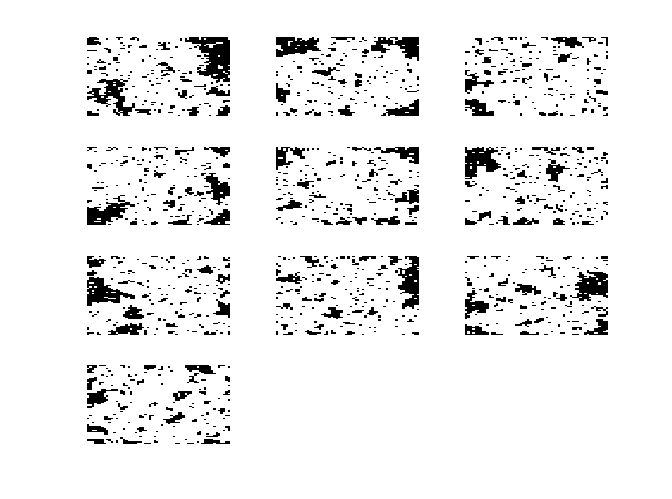
\includegraphics[width=0.4\textwidth]{Images/block_1.png}
    \hfill
	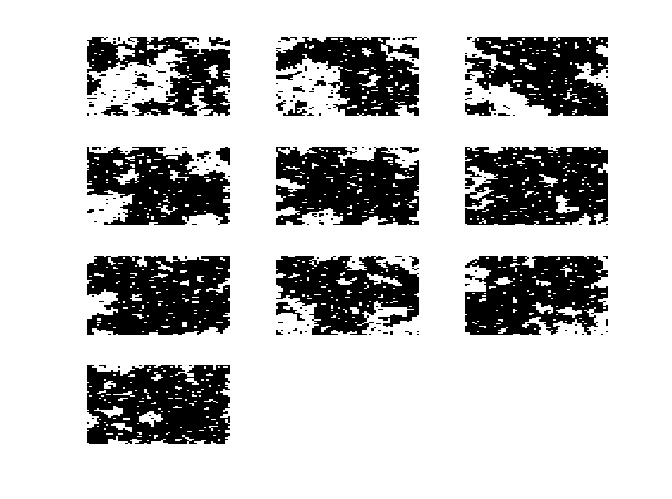
\includegraphics[width=0.4\textwidth]{Images/block_3.png}
    \caption{Two samples generated by block gibbs sampler} 
\end{figure}

\begin{figure}[htbp]
  \centering
    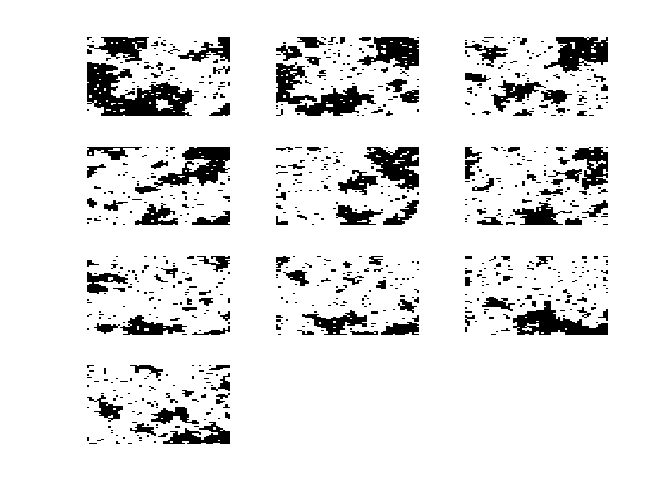
\includegraphics[width=0.4\textwidth]{Images/gibbs_sampler_1.png}
    \hfill
	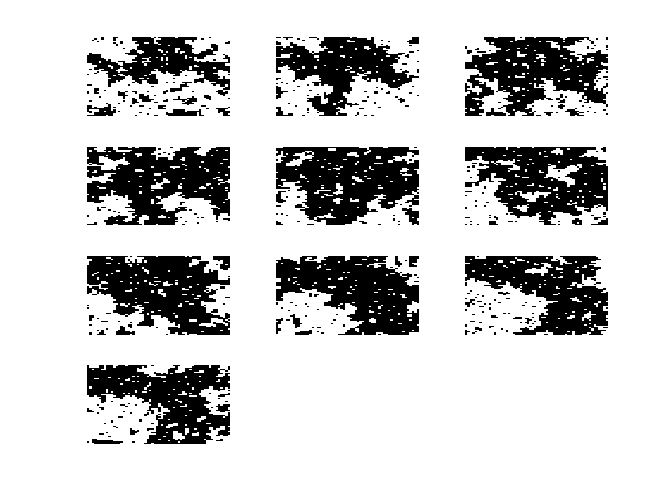
\includegraphics[width=0.4\textwidth]{Images/gibbs_sampler_2.png}
    \caption{Two samples generated by our gibbs sampler} 
\end{figure}


From the above observations it seems that the block gibbs sampler has a lower mixing time. This become even more apparent when we look at extreme values of $\theta$ such as $\theta=100$ where the block gibbs sampler converges in just 3 iteration while our gibbs sampler takes 6.

\begin{figure}[htbp]
  \centering
    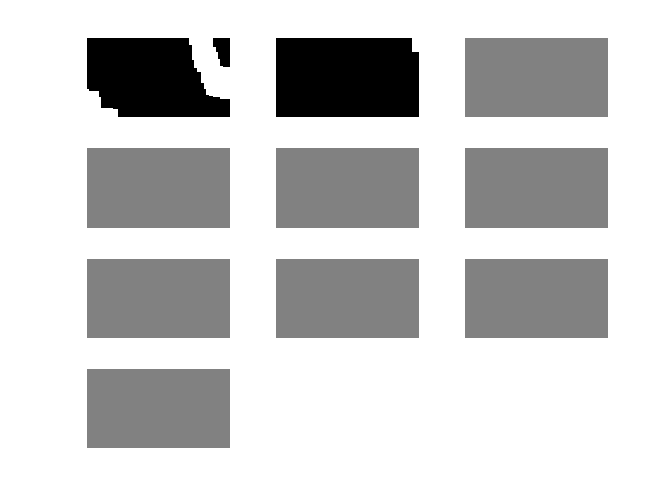
\includegraphics[width=0.4\textwidth]{Images/block_theta_100.png}
    \hfill
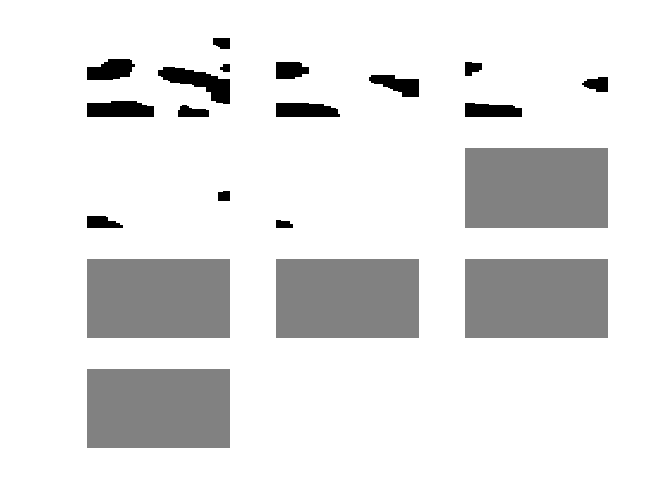
\includegraphics[width=0.4\textwidth]{Images/gibbs_sampler_theta_100.png}
    \caption{Comparison of mixing time for block (left) and our Gibbs sampler (right) for $\theta=100$}
\end{figure}
\end{document}